\subsection{Opportunities with the deuteron}

The deuteron is the lightest non-trivial nucleus and it has a wave function dominated by a loosely bound proton--neutron configuration.  As such, it offers a range of possibilities to study QCD phenomena at hadronic and partonic scales.  As it offers a (bound) neutron target, DIS off a deuteron is together with PVDIS the main tool to perform flavor separation of quark distribution functions.  As a bound $pn$ system, it also offers a window into the QCD origin of the nucleon-nucleon force and medium modifications of nucleon properties~\cite{Boeglin:2015cha}.  In kinematics where a high-energy probe interacts with both nucleons in the deuteron, coherent phenomena in QCD such as shadowing and saturation can be studied.  Lastly, the deuteron is a spin-1 hadron and as a result studies with a polarized deuteron offer additional observables and opportunities beyond those of the free polarized nucleon.

When inclusive DIS is carried out on a nucleus, the process averages over all initial configurations.  This means one has to account for possible medium modifications and include binding effects and non-nucleonic degrees of freedom in the nuclear wave function.  A handle on the control of the initial state of the target nucleus is provided by the spectator tagging process, where a slow nucleon (relative to the center of mass of the nucleus) is detected in the target fragmentation region of the final state.  For the deuteron, controlling the initial target state through spectator tagging has several advantages.  Spectator tagging effectively identifies the active nucleon participating in the DIS reaction (proton tagging enables neutron structure studies and the other way around) and suppresses nuclear binding effects at low spectator momenta. 

By varying the momentum of the detected spectator, one can also select compact (high momentum) or loose configurations (low momentum) of the deuteron (see Fig.~\ref{fig:size}).  This allows the study of nuclear binding effects and the nature of the $NN$-interaction at different length scales and densities.  Of course, one has to account for the possible final-state interactions (FSIs) between the spectator and the DIS products.  The deuteron has the advantage there is only one possible spectator nucleon, meaning FSIs are tractable.  Moreover, in kinematics with large FSIs they can be used to obtain information about the process of hadronization in the DIS products~\cite{Cosyn:2017ekf}.  

The deuteron also has the advantage that first principles non-relativistic wave functions are available to perform theoretical calculations.  In high-energy reactions, the structure of the light-front deuteron wave function is known~\cite{Frankfurt:1981mk,Keister:1991sb} and it can be matched to the non-relativistic wave functions at small relative momenta.

    \begin{figure}
        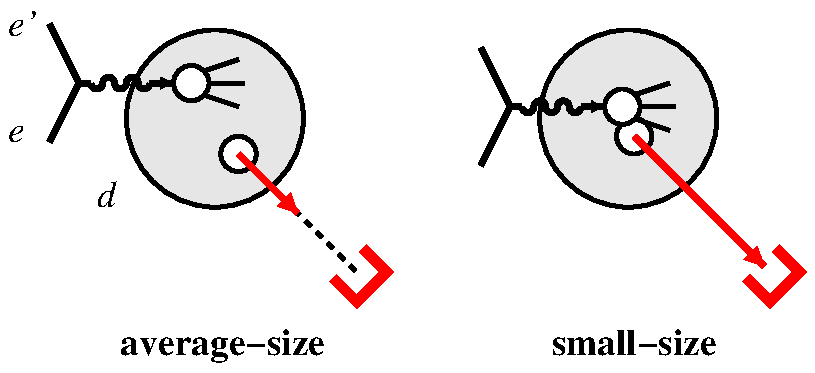
\includegraphics[width=0.5\textwidth]{plots/deut_tag_restframe}
        \caption{Deuteron lab frame depiction of the spectator tagging process.  Low spectator momenta select average-sized configurations, large spectator momenta access small-sized ones~\cite{deutLDRD}}
        \label{fig:size}
    \end{figure}

To access on-shell nucleon structure, the technique of pole extrapolation can be applied to the spectator tagging process.  Here, observables as a function of spectator momentum are extrapolated in the unphysical region to the on-shell point of the active nucleon.  The small binding of the deuteron implies the extrapolation length into the unphysical region is quite small, resulting in controllable errors on the extrapolated values.  The no-loop theorem implies that although higher order diagrams (suchs as FSIs) contribute to the spectator tagging process, they do not contribute at the on-shell point~\cite{Sargsian:2005rm} implying the access to free neutron structure functions for proton tagging.  Additionally, at the on-shell point the deuteron polarization is almost 100\% transferred to both nucleons due to the deuteron $S$-wave dominance, enabling the extraction of on-shell neutron spin structure in spectator tagging with polarized beams.  

Spectator tagging on the deuteron has been measured at JLab at both high (DEEPS experiment~\cite{Klimenko:2005zz}) and low spectator momenta (BoNuS experiment~\cite{Baillie:2011za}). In a fixed target setup this measurement is challenging, especially at low spectator momenta. Hence a dedicated detector had to be installed in the BoNuS experiment.  These difficulties disappear for an electron-ion collider, where the spectators still move forward after the DIS event with momenta of the order of half the deuteron beam momentum, and can be detected in forward detectors (see Fig.~\ref{fig:collider}).  Together with the wide kinematic range in Bjorken $x$ and $Q^2$ that an EIC offers, spectator tagging can make a significant impact on on-shell neutron structure data and studies of medium modifications.  Extensions of the tagging process are also possible using light nuclei beams beyond the deuteron and measuring more exclusive channels.  The theoretical framework and simulation tools for the spectator tagging process are under active development~\cite{deutLDRD,Guzey:2014jva,Cosyn:2016oiq} and estimates for the size of FSIs at an EIC have recently been provided~\cite{Strikman:2017koc}.

    \begin{figure}
        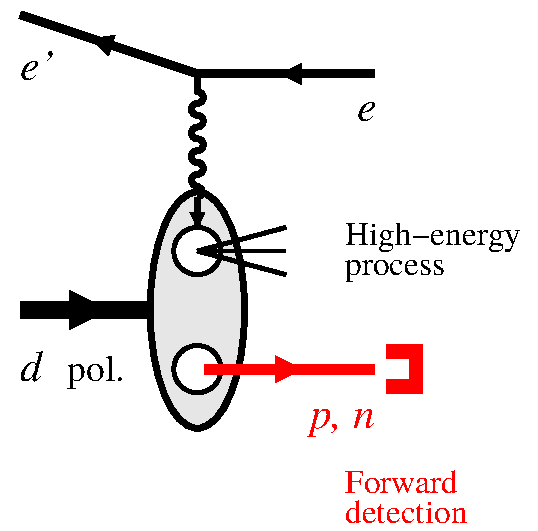
\includegraphics[width=0.28\textwidth]{plots/deut_tag_collider}
        \caption{Collider frame depiction of the spectator tagging process with forward detectors capturing the spectator nucleon~\cite{deutLDRD}}
        \label{fig:collider}
    \end{figure}

A straightforward way of probing the additional spin degrees of freedom the deuteron offers is by performing inclusive DIS off a tensor polarized target, which is sensitive to four additional structure functions~\cite{Hoodbhoy:1988am}.  One of these $b_1$ has an interpretation in the parton model as a linear combination of unpolarized quark PDFs in a polarized spin-1 hadron
\begin{equation}
b_1=\frac{1}{2}\sum_q e_q^2(q^0-q^1)\,,
\end{equation}
where $q^i$ is the quark PDF in a hadron with polarization $i$ along the virtual photon momentum.  Hence, $b_1$ probes the interplay of nuclear and quark degrees of freedom.  Currently, there exists only one measurement of $b_1$ from HERMES~\cite{Airapetian:2005cb} that cannot be explained by conventional deuteron convolution models.  A new measurement is planned at JLab~\cite{Slifer:2013vma}, which spurred updated convolution model calculations~\cite{Cosyn:2017fbo} and estimates of hidden color and pion cloud contributions~\cite{Miller:2013hla}.
